\documentclass[a4paper,11pt]{article}
\usepackage{amssymb}
\usepackage{booktabs}
\usepackage{geometry}
\usepackage{color}
\usepackage{hyperref}
\usepackage{listings}
\usepackage{graphicx}
\usepackage{float}
\usepackage{caption}
\usepackage{subcaption}
\usepackage[T1]{fontenc}


\graphicspath{{img/}}

\setlength\parindent{0cm}

\geometry{
	includeheadfoot,
	margin=2.54cm
}

\title{
	2IL76 Algorithms for Geographic Data Set 4 \\
}
\author{
	Tim van Dalen (0744839)
	\and
	Bram Kohl (0746107)
	\and
	Bart van Wezel (0740608)
}
\date{\today}

\begin{document}
	\maketitle
	
\section*{Exercise 3}
For every region that is (partially) within the necklace, we place a point on the necklace as close as possible to the center of the (full) region.
We then combine the points of the regions of the same type by calculating a point between them, which is weighted by the area the region takes within the necklace.
The final circle on the necklace is placed as close as possible to this point.

\paragraph{Example} There are 3 regions of type X which have a part in the necklace. \\
We first determine for each region: a point on the necklace, such that the distance to the center of the region is the lowest.
In this example, as can be seen in Figure~\ref{fig:example}, we have points $A,B,E,F$.  \\

Then, for the types that have more than one region in the necklace, we determine the factor for each region.
We do this by dividing the size of that region, by the total size of that type. 
So, for the left-most yellow region, this factor is $\frac{4}{5}$.
For the right yellow region, the factor is $\frac{1}{5}$.

Now, for each region, we multiple the point on the necklace by the factor for that region.
We then take the sum of all points per type.
Thus, for the left yellow region, we found the point $(1,0.5)$ on the circle and factor $\frac{4}{5}$.
The point for this region is then $(0.8,0.4)$.
For the right yellow region, we found the point $(2,2)$ on the circle and factor $\frac{1}{5}$.
This points becomes $(0.4,0.4)$.
Taking the sum of these points, we get point $C$, at $(1.2,0.8)$.
From this point, we will again determine a point on the necklace, such that the distance to point $C$ is the lowest. \\
In this example, that is point $D$.

For each type, we place the ring belonging to that type on the selected point on the necklace.
For the yellow type, this is point $D$.
Since the red and the blue types only have one region, their rings are placed simply on $E$ and $F$, respectively.

\begin{figure}[H]
	\centering
	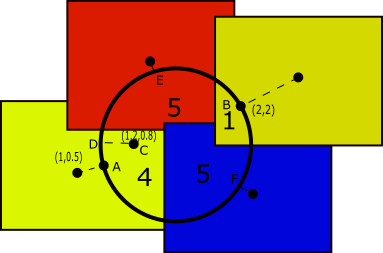
\includegraphics{figure1.png}
	\caption{Example describing our model}
	\label{fig:example}
\end{figure}

When the rings of multiple regions intersect, we move the outer rings away untill they can be placed without intersection.
For example, when three rings intersect, we move the two outer rings away.
When two rings intersect we move away both rings till they can be placed without intersection. 
When there are more than three rings that intersect, we first move the outer two away and repeat this process untill there are no intersections left.

We can continously move the circle, while still being spatially informative. 
When new regions join the necklace or old regions leave the necklace, they only take into account a small part of the total size of that type. 
This is because when a new region enters the necklace at first only a small part of that region is in the necklace and thus the factor of that region is still small. 
If we move the circle further into that region, the factor increases and the label for that type changes its location slowly to that new region, given that that region is of significant size.
Before a region leaves the necklace, the part of the region that is inside the necklace will become continuously smaller.
Because of this, the factor for that region also becomes smaller, meaning that the weight of that region on the position of the ring becomes smaller.
This means the ring for the type of that region has already moved towards its new position.

\end{document}


